\begin{anexosenv}

  \partanexos

  \chapter{Diagrama de Classes Backend}
  \label{anx:server_uml}
  Diagrama de classes do backend na figura \ref{fig:server_uml}, desenvolvido no projeto UMISS.
  \begin{figure}[!h]
    \centering
    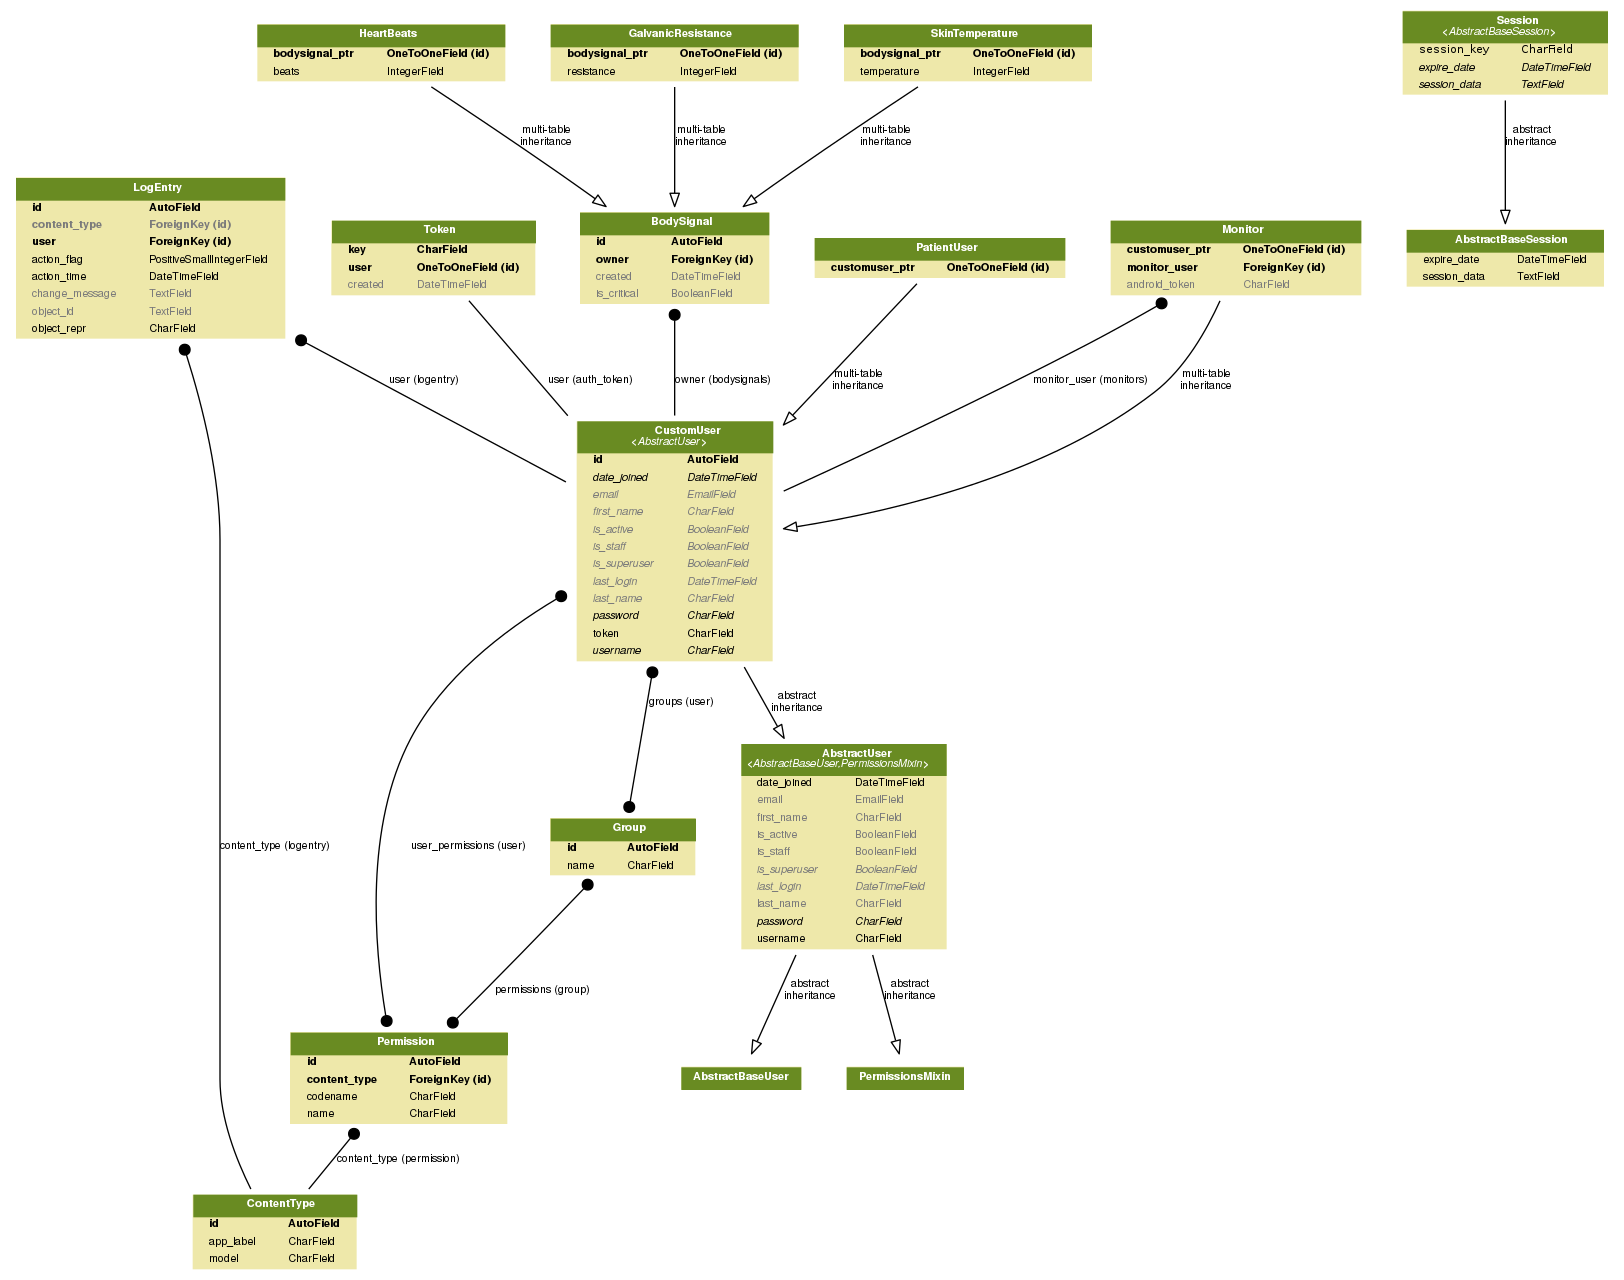
\includegraphics[width=\textwidth, angle=90]{figuras/server_uml.png}
    \caption{\textit{Design} e Arquitetura do servidor Django}
    \label{fig:server_uml}
  \end{figure}

  \chapter{Teste de Bancada}

      \section{Dobrador de tensão:}

      aqui tem um texto

      \section{Chaveamento:}

      Para o teste de bancada do chaveamento do circuito foi utilizado uma bateria de 9V como fonte de alimentação para o dobrador de tensão e o Arduino foi utilizado aqui como plataforma com o microcontrolador, em que o código para controle por joystick e ativamento do PWM (1 kHz) e sentido da corrente eram executados pelo microcontrolador. Foi utilizado a bateria de 9 V devido o teste de bancada do chaveamento ter sido realizado em casa, mas mesmo com 9 V o circuito é capaz de realizar suas funções sem maiores problemas. Um ponto a citar aqui é que o valor do dobrador de tensão não está em 18 V devido a bateria não estar totalmente completa em carga, portanto o valor menor nos testes, gerando assim quedas de tensão menores para as saídas do chaveamento, mas mesmo assim ainda corretas.

      Vale destacar também que ao se ligar os sentidos das correntes de acordo com o desejado, as saídas cumpriram seu dever, executando o planejado para o chaveamento. As figuras aqui apresentadas para os testes não mostram as saídas  quando solicitadas para desligamento de algum sentido da corrente, apenas apresentam quando solicitadas para ligamento de algum sentido da corrente.

      \begin{figure}
          \begin{center}
              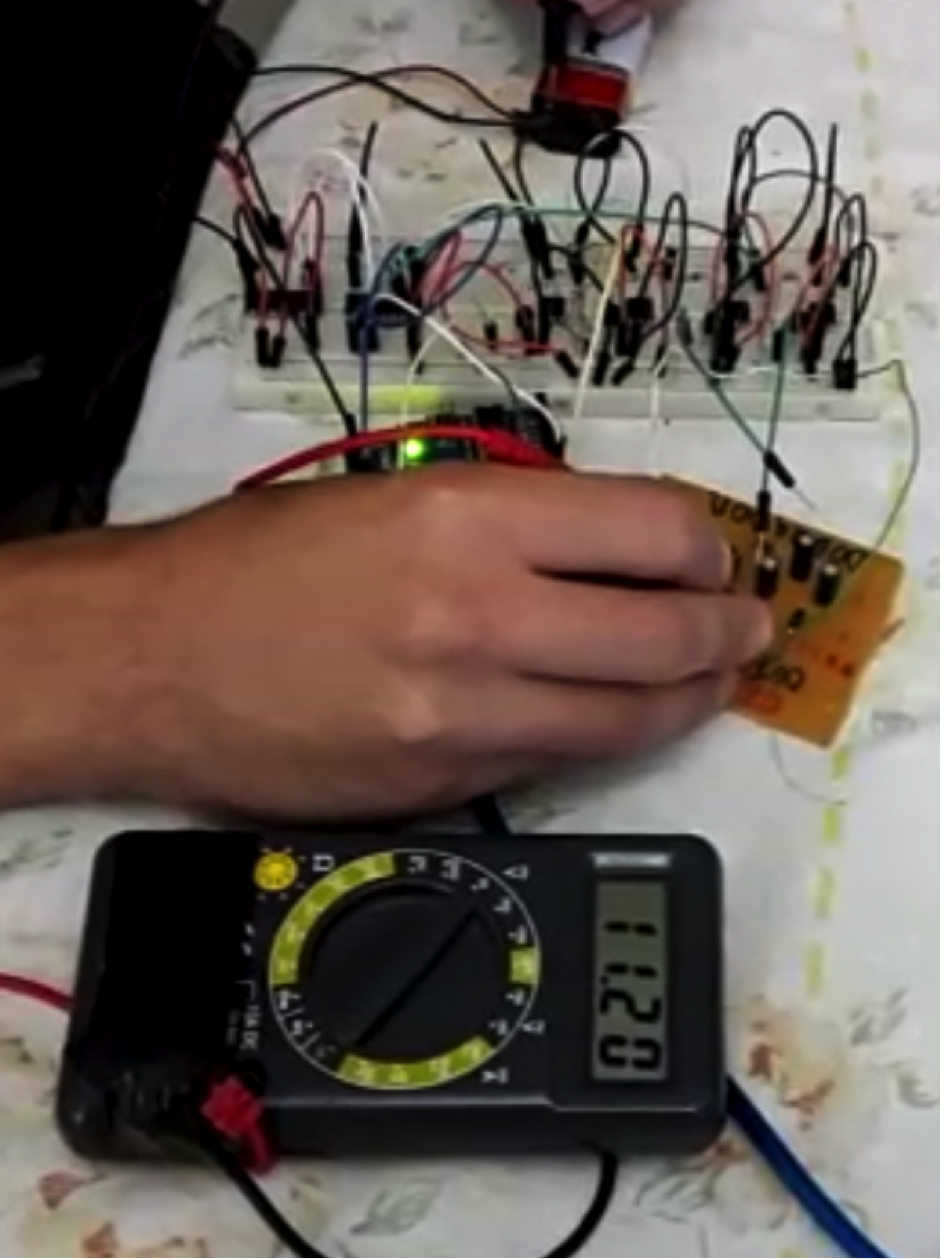
\includegraphics{figuras/teste_alimentacao_1.png}
          \end{center}
          \caption{Valor do dobrador de tensão para o  teste de chaveamento.}
          \label{fig:teste_alimentacao_1.png}
      \end{figure}

      \begin{figure}
          \begin{center}
              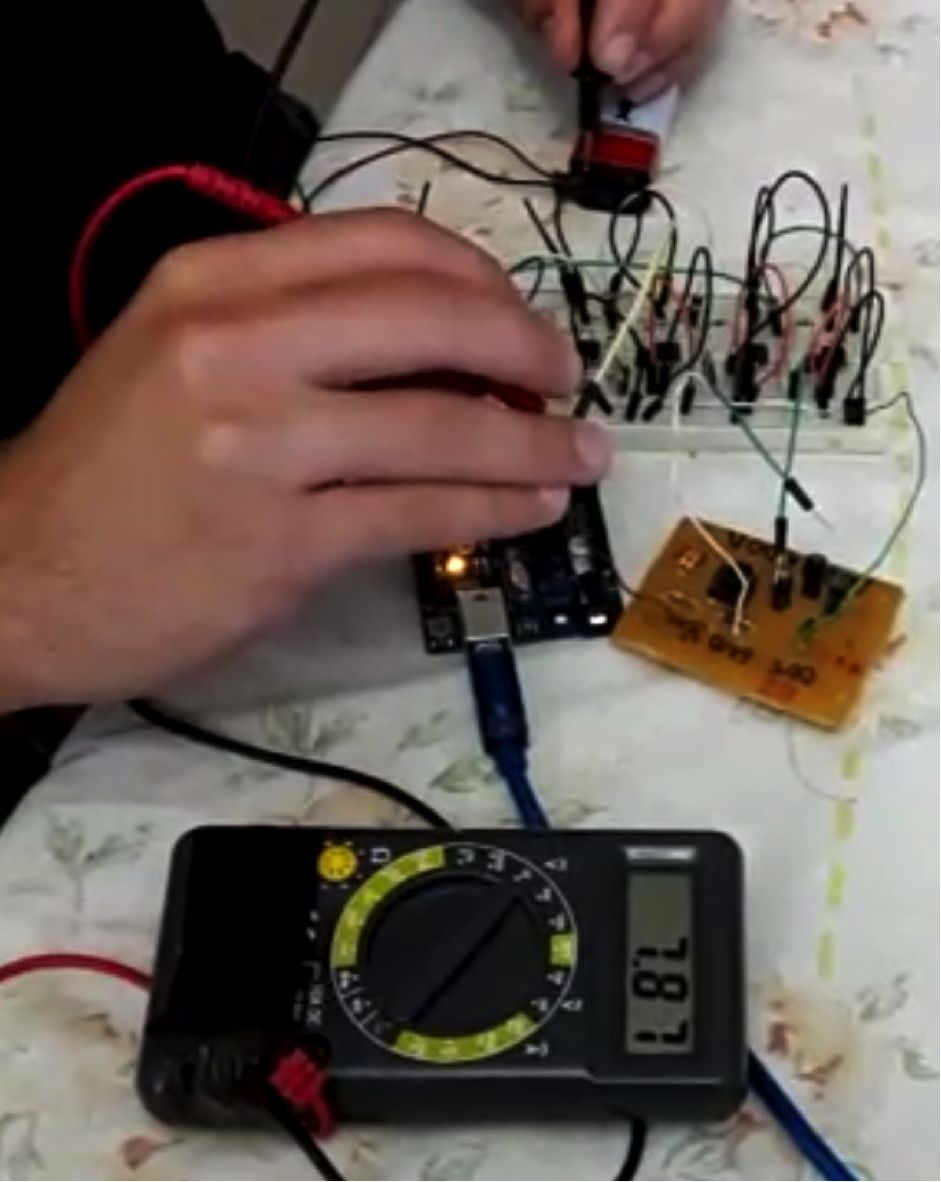
\includegraphics{figuras/teste_alimentacao_2.png}
          \end{center}
          \caption{Teste da saída para o transistor MOSFET Q1 (sentido direto).}
          \label{fig:teste_alimentacao_2.png}
      \end{figure}

      \begin{figure}
          \begin{center}
              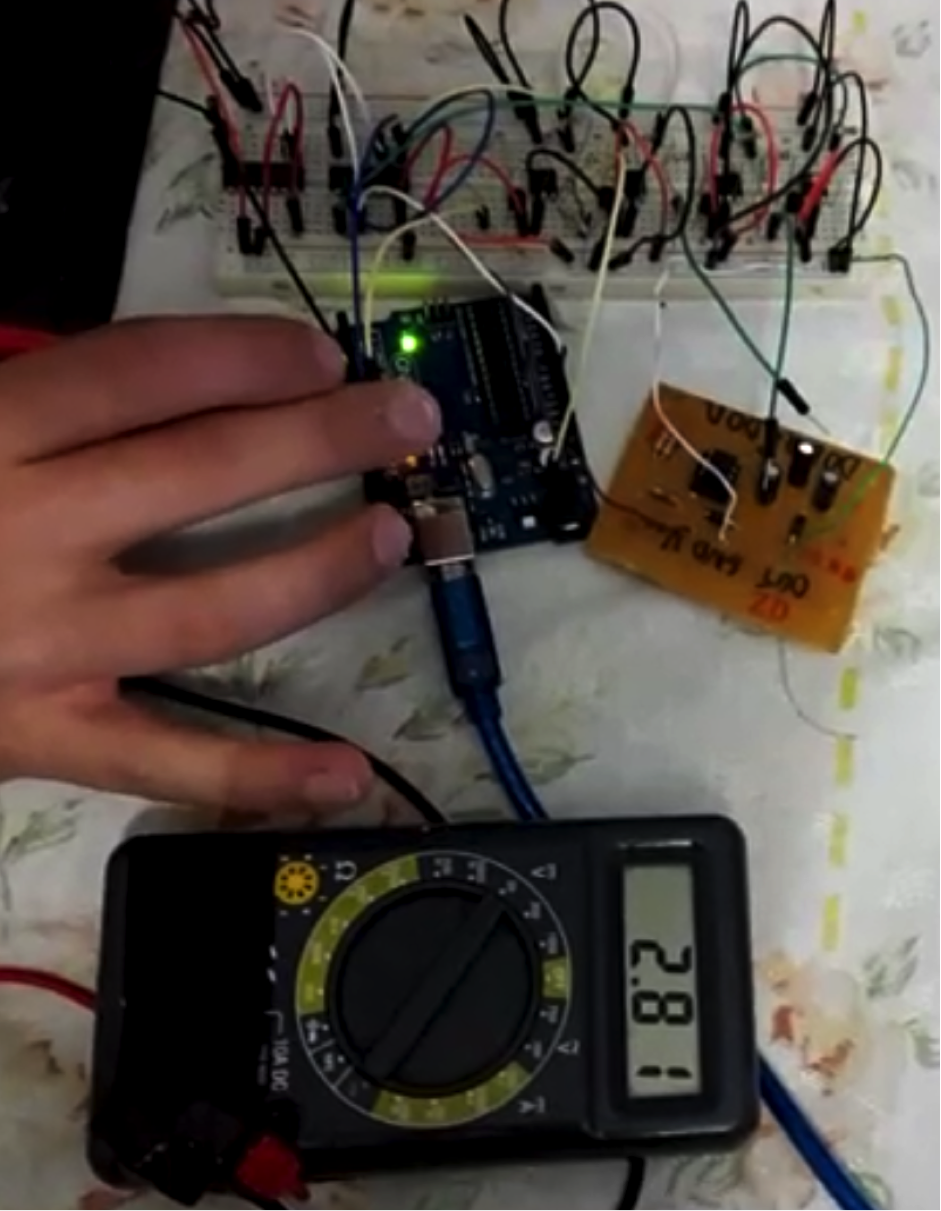
\includegraphics{figuras/teste_alimentacao_3.png}
          \end{center}
          \caption{Teste da saída para o transistor MOSFET Q4 (sentido direto).}
          \label{fig:teste_alimentacao_3.png}
      \end{figure}

      \begin{figure}
          \begin{center}
              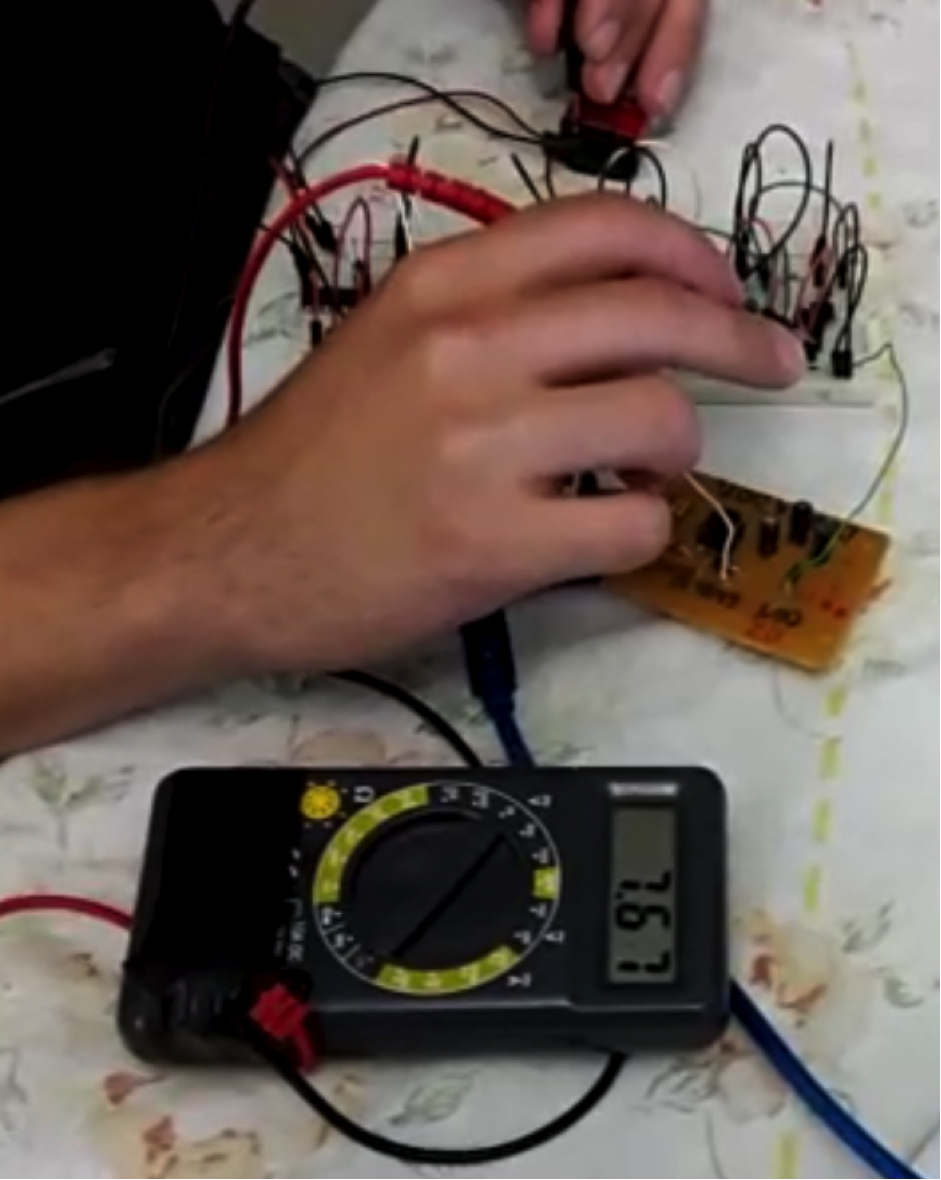
\includegraphics{figuras/teste_alimentacao_4.png}
          \end{center}
          \caption{Teste da saída para o transistor MOSFET Q3 (sentido inverso).}
          \label{fig:teste_alimentacao_4.png}
      \end{figure}

      \begin{figure}
          \begin{center}
              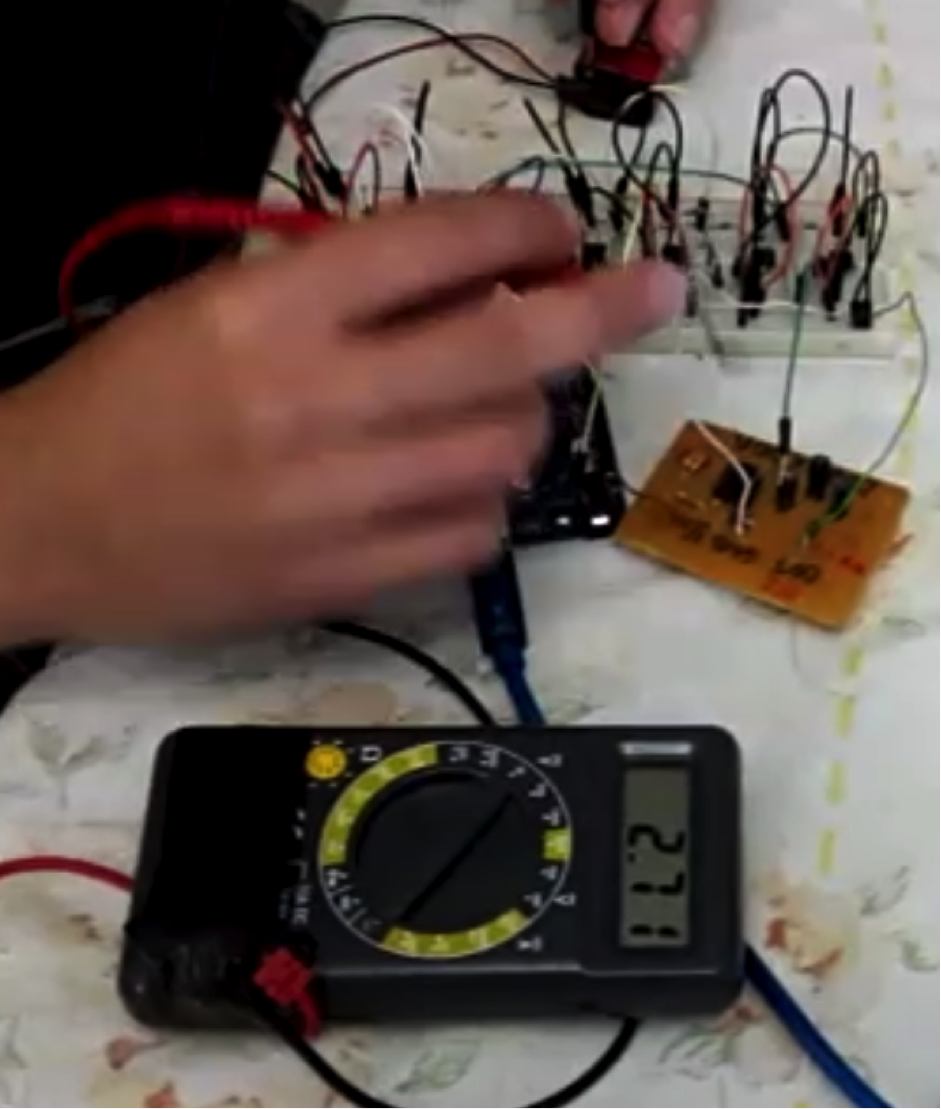
\includegraphics{figuras/teste_alimentacao_5.png}
          \end{center}
          \caption{Teste da saída para o transistor MOSFET Q2 (sentido inverso).}
          \label{fig:teste_alimentacao_5.png}
      \end{figure}

      \section{Ponte H}

      aqui tem texto

      \section{PWM}

      AQUI TEM MAIS TEXTO









\end{anexosenv}
